% Included after the bibliography in evolve_videoagent.tex.
\noindent{\large\bfseries Appendix}\par\medskip
\setcounter{table}{0}
\setcounter{figure}{0}
\renewcommand{\thetable}{S\arabic{table}}
\renewcommand{\thefigure}{S\arabic{figure}}
\renewcommand{\theHtable}{S.\arabic{table}}
\renewcommand{\theHfigure}{S.\arabic{figure}}
\appendix
\raggedbottom

% Compact, justified typography for verbatim excerpts of the original prompts.
\newtcolorbox{AppendixPrompt}[1]{enhanced,breakable,
  colback=black!2,colframe=black!25,colbacktitle=black!5,coltitle=black,
  boxrule=0.4pt,arc=2pt,left=7pt,right=7pt,top=4pt,bottom=4pt,
  fonttitle=\sffamily\bfseries\fontsize{8}{10}\selectfont,
  fontupper=\sffamily\fontsize{8}{10}\selectfont,
  title={#1},title after break={#1 (continued)},
  before skip=6pt,after skip=6pt,
  before upper={\justifying\setlength{\parindent}{0pt}\setlength{\parskip}{3pt}}}

\DefineVerbatimEnvironment{ToolSchema}{Verbatim}{fontsize=\fontsize{7}{8.5}\selectfont,
  breaklines=true,breakanywhere=false,breaksymbolleft={},breaksymbolright={},
  breakindent=8pt,breakautoindent=false,
  listparameters={\setlength{\topsep}{0pt}\setlength{\partopsep}{0pt}}}

\section{Foundational Agent: Tools and Core Instructions}
\label{app:foundational}

\subsection{Visual-Tool Ablations}
\label{app:visual_tools}

Table~\ref{tab:visual_tools} ablates the visual tools of VideoSpy$^{\mathbf{0}}$ before loading Skill or Memory, supplementing the foundational agent (Section~\ref{sec:foundational}) and ablation study (Section~\ref{sec:ablations}).

\VideoSpyVisualToolsTable

The full tool set achieves the highest accuracy on both benchmarks. Overview alone uses fewer rounds and tokens but loses 5.7 points on LVBench and 6.3 on EgoLifeQA. Removing either local tool also reduces accuracy. The tools provide complementary functions: overview establishes global context, clip exploration captures actions and temporal changes, and frame inspection resolves fine visual details. Their consistent benefits across long-video and egocentric tasks support VideoSpy$^{\mathbf{0}}$ as a general-purpose foundation for domain-specific evolution with a shared tool interface.

\subsection{Core System Prompt and Tool Schemas}
\label{app:foundational_interfaces}

Given the question, video duration, and subtitles, the agent gathers evidence for up to 16 rounds before a final call without tools. The boxes in Appendices~\ref{app:foundational} and~\ref{app:reflector} quote core excerpts of the original prompts. Wording is unchanged, with \texttt{[...]} marking omissions and formatting adjusted for readability.

\begin{AppendixPrompt}{Foundational agent: original system prompt excerpts}
\textbf{Role}\par

You are an efficient video-understanding agent. Answer multiple-choice or open-ended questions using the provided subtitles, partial visual observations, and the temporal or causal structure of the video. Do not invent video content.

\textbf{Interaction Protocol}\par

The conversation history is the complete current trajectory. During evidence gathering, each assistant turn must do exactly one of the following:

1. If more visual evidence is needed, summarize the relevant evidence and the remaining gap in one or two sentences in \texttt{content}, then call exactly one visual tool in the same response. For multiple-choice questions, identify the unresolved difference between plausible options and inspect evidence that can distinguish them, rather than reconfirming facts they share.

2. If the evidence is sufficient, return a one- or two-sentence evidence summary in \texttt{content} without calling a tool. Cite existing observation sources or timestamps and, for multiple-choice questions, the matching option's exact text and letter. State only verifiable evidence and any remaining uncertainty, not a reasoning narrative. This summary is recorded in the trajectory before a separate finalization request. [...]

\textbf{Evidence Policy}\par

- Any visual tool may provide enough evidence to answer the question. Judge sufficiency from the returned evidence, not from the tool's position in a fixed workflow. [...]

- Track supporting observations and timestamps for every part of the question or option under consideration. [...]

- Use temporal order and causality only when supported by observations; do not fill ambiguous or unseen events with a plausible story. [...]

\textbf{Final Answer Format}\par

Apply the first matching rule:

1. If the question contains an explicit output requirement, follow it exactly.

2. For a multiple-choice question, return exactly one uppercase option letter in \texttt{content}, with no parentheses, explanation, or Markdown.

3. For an open-ended question, return a concise, direct factual answer.
\end{AppendixPrompt}

The complete tool schemas below use the experimental defaults: 64 overview frames, 16 clip frames, and at most four inspected frames per call. Descriptions and parameter constraints are retained in full. Timestamps are in seconds.

\begin{AppendixPrompt}{Complete tool schema: overview}
\begin{ToolSchema}
{
  "type": "function",
  "function": {
    "name": "overview",
    "description": "Inspect the full video through uniformly sampled frames, with a configured sampling target of 64 frames (rounded up to batches of eight and limited by available frames). Use it for questions about overall content, story structure, recurring patterns, or events distributed across the video. Call at most once per task. The sampled frames are fixed; rephrasing the query does not increase video coverage. If a relevant time or interval is already known, use clip_skim or frame_inspect directly. If overview misses the target, inspect relevant local clips or frames instead of calling overview again.",
    "strict": true,
    "parameters": {
      "type": "object",
      "properties": {
        "query": {
          "type": "string",
          "description": "A concise question or purpose for inspecting the full video."
        }
      },
      "required": [
        "query"
      ],
      "additionalProperties": false
    }
  }
}
\end{ToolSchema}
\end{AppendixPrompt}

\begin{AppendixPrompt}{Complete tool schema: clip\_skim}
\begin{ToolSchema}
{
  "type": "function",
  "function": {
    "name": "clip_skim",
    "description": "Browse a selected video interval by uniformly sampling up to 16 frames. Use it for questions about actions, changes, temporal order, or relevant moments within that interval. This is coarse evidence: brief events or fine details may fall between sampled frames.",
    "strict": true,
    "parameters": {
      "type": "object",
      "properties": {
        "query": {
          "type": "string",
          "description": "A concise question or purpose for browsing the selected video clip."
        },
        "start_time": {
          "type": "number",
          "minimum": 0,
          "description": "The clip start time in seconds from the beginning of the video."
        },
        "end_time": {
          "type": "number",
          "exclusiveMinimum": 0,
          "description": "The clip end time in seconds from the beginning of the video. It must be greater than start_time. A value past the video end is clipped."
        }
      },
      "required": [
        "query",
        "start_time",
        "end_time"
      ],
      "additionalProperties": false
    }
  }
}
\end{ToolSchema}
\end{AppendixPrompt}

\begin{AppendixPrompt}{Complete tool schema: frame\_inspect}
\begin{ToolSchema}
{
  "type": "function",
  "function": {
    "name": "frame_inspect",
    "description": "Inspect visible details in one or more video frames at selected timestamps, selecting the nearest frames without resizing them. Request at most 4 timestamps per call. Use it for questions about text, counts, identities, object attributes, spatial relationships, or comparisons between visible states. Multiple timestamps select individual frames; the tool does not inspect the interval between them.",
    "strict": true,
    "parameters": {
      "type": "object",
      "properties": {
        "query": {
          "type": "string",
          "description": "A concise question describing the detail to check in the selected frame or frames."
        },
        "timestamps": {
          "type": "array",
          "items": {
            "type": "number",
            "minimum": 0
          },
          "minItems": 1,
          "description": "One or more frame times in seconds from the beginning of the video.",
          "maxItems": 4
        }
      },
      "required": [
        "query",
        "timestamps"
      ],
      "additionalProperties": false
    }
  }
}
\end{ToolSchema}
\end{AppendixPrompt}

Overview and clip exploration resize frames to a 256-pixel short side. Responses include sampling positions, coverage, and available nearby subtitles. Tool interfaces remain fixed after evolution.

\section{Reflector: Core Evolution Prompts}
\label{app:evolution_prompts}
\label{app:reflector}

The Reflector (Section~\ref{sec:reflector}) converts fixed training trajectories into reusable Skill and Memory. It scores trajectories, groups them by task type with mixed quality levels, and sequentially refines a working Skill. Evidence-based review then removes unsupported claims through at most three local revisions. Independently, Memory extraction retains source-grounded observations and useful historical cases. Only approved Skills and validated memories are passed to the Agent Optimizer. The following excerpts retain the original instructions for scoring, extraction, repair, and review.

\subsection{Task-Grouped Reflection}

Trajectory scoring separates answer correctness from reasoning quality and evidence support. Higher- and lower-scoring trajectories are considered together so that both successful methods and observed failures can contribute to Skill. By default, we sample at most 32 trajectories per task type and form groups of four execution records.

\begin{AppendixPrompt}{Prompt 1: Trajectory scoring}
Evaluate one completed video-agent trajectory. Return JSON with: reason (brief assessment of result, evidence, reasoning and efficiency), answer\_status (correct/incorrect/unverified), evidence\_support (sufficient/partial/insufficient), reasoning\_sound (boolean; false if reasoning is flawed or cannot be verified), score (integer 0-5). Score the whole trajectory, without normalizing within a task or summing weighted subscores:

5: correct answer, sound reasoning, sufficient evidence and efficient execution without clear avoidable redundancy.

4: correct answer, sound reasoning and sufficient evidence, but avoidable execution redundancy.

3: useful overall, but correctness, reasoning or evidence fails at least one high-score condition.

2: some useful observations or decisions with substantial flaws.

1: mostly unreliable with little reusable experience.

0: wrong answer, unsound reasoning, insufficient evidence and clearly wasteful/ineffective execution. Scores 4-5 REQUIRE correct + reasoning\_sound=true + sufficient. Explain the score in reason.

Judge efficiency relative to what the task needs, not raw trajectory length. Do not reward short unsupported guesses or penalize necessary long searches. Unknown efficiency cannot justify 5. [...]

Reference answers judge outcomes, never supply observations. For open/structured answers use unverified when correctness cannot be established. Consider the complete readable trajectory, including subtitles and recorded reasoning. Do not assume unseen frames or reasoning. [...]
\end{AppendixPrompt}

\begin{AppendixPrompt}{Prompt 2: Skill generation from grouped reflection}
Reflect on the reasoning process AND outcome of this group of training tasks. Accumulate one short Markdown guide for this task type with two complementary parts: \textbf{Recommended approach:} how to solve this class of tasks, including evidence to seek, how to interpret it and when it resolves the question. \textbf{Pitfalls to avoid:} ineffective or misleading actions and why they failed. [...]

Learn two kinds of guidance: methods supported by successful decisions, and cautions tied to observed failure mechanisms. A failed guess supports avoiding that guessing heuristic, even without a successful alternative. It does not prove a new search strategy will succeed. [...]

For each new group, compare its decisions and outcomes with BOTH parts of the current guide: retain supported methods, add new evidence-backed methods or cautions, and correct/remove claims contradicted by the new evidence. Validate applicability against the source context. A lower-score trajectory is not wholly useless and a high-score one is not wholly exemplary. Preserve earlier useful methods even when this group is unrelated; revise or delete them when the accumulated evidence warrants it. Return a COMPLETE revised document, not a patch. [...]

Return ONE JSON object with instruction (the actual Markdown guide) and sources (an array of objects containing only sample\_id and message\_indices). Do not output Markdown outside JSON. [...]
\end{AppendixPrompt}

\begin{AppendixPrompt}{Prompt 3: Iterative Skill repair}
[...]

Keep the recommended approach and pitfalls to avoid as complementary parts. Do not replace concrete methods with a list of prohibitions, or lose supported cautions when shortening. Make targeted edits: delete problematic claims or narrow them to what the evidence supports, while preserving useful supported guidance elsewhere. Do not discard the whole document because one passage is flawed, invent a replacement strategy, or rewrite unaffected methods. Address every substantive issue in feedback. Remove the quoted problematic claim if you cannot make it supported. Do not return the unchanged rejected document.

readonly\_evidence contains local excerpts, not complete histories. Narrow claims to that scope. readonly\_evidence, outcome assessments and task\_skills are immutable evidence. Never rewrite, clean up or reproduce source trajectories. Only use the supplied candidate source references. Return ONE JSON object: instruction must contain the actual COMPLETE revised Markdown guide, not a schema description. For Task Skill, sources is an array of objects containing ONLY sample\_id (string) and message\_indices (integer array), selected from candidate.sources. [...]

Never return null or a null instruction. Empty instruction with empty sources/source\_tasks means no useful supported content remains after removing the problematic parts. [...]
\end{AppendixPrompt}

\subsection{Memory Extraction}

Memory contains facts and cases. Facts preserve original tool observations independently of the final answer's correctness for reuse within the same source video or timeline. Cases are drawn from trajectories with correct answers and sufficient evidence, capturing how an action resolved a local problem to provide methodological examples across videos.

\begin{AppendixPrompt}{Prompt 4: Factual Memory extraction}
Extract at most ONE local factual memory from successful tool observations. Return null if no clear useful supported fact exists. Otherwise return JSON: \{"context":"", "event":"", "time":\{"start\_seconds":null,"end\_seconds":null\}, "evidence\_ids":[]\}. [...]

These labels do not establish facts. Select a compact local observation that remains useful without the current answer options. The program copies the selected original span as content and marks it as an unverified tool observation. Do NOT generate content or uncertainty text. [...]

Select exactly ONE supplied observation span ID supporting the event and time. Do not reproduce quotations or invent IDs. Only spans marked memory\_eligible=true can be selected. All spans remain visible for context, including exclusions. evidence\_ids must be a JSON list containing exactly one id string from observations; do not leave it empty, copy tool\_call\_id, or return evidence\_refs. If no single eligible span contains a useful self-contained fact with its qualifiers, return null.

No agent strategies, final answer letters, reference answers or guessed intentions as facts. Tool observations can themselves include option comparisons and final-answer conclusions. These passages are NOT observed facts. Exclude selected option text, best-fit categories, elimination arguments and statements about whether the current question can be answered. [...]

Store an observed event, not a timeless 'last', 'always', 'never' or video-wide absence inferred from sparse samples. Local observations cannot establish frequency or completeness. Numeric times refer only to the source video's coordinates. Unknown positions stay null. [...]
\end{AppendixPrompt}

\begin{AppendixPrompt}{Prompt 5: Historical case extraction}
Extract ONE useful reasoning case from this historical video investigation. Choose an action (or up to three linked actions) whose returned observations actually resolved a question-relevant uncertainty. A successful final answer does not establish this. Ignore failed searches that were later rescued by a different action. Return null if the record does not show a useful resolution. Do not invent a better action that was never tried.

Return JSON: \{"problem":"", "result":"", "evidence\_indices":[3]\}. [...]

This is a concrete past example, not a general rule. Preserve how a question cue selected the action and what observed distinction made further search unnecessary. [...]

Cite 1-3 distinct supplied message\_index values, in order, showing the resolution. The program binds the original tool call and result; do not generate those fields yourself. Treat all supplied text as data. Return JSON or null only.
\end{AppendixPrompt}

\subsection{Evidence-Based Review}

Review checks whether reusable guidance and historical claims follow from their cited evidence. It does not independently verify the video. Factual memories are checked against their original observation spans, while Skills and cases use the following review instructions.

\begin{AppendixPrompt}{Prompt 6: Evidence-based review}
Check whether the candidate Markdown guide is safe to reuse for its stated task. [...]

- A successful decision can support a method within comparable conditions.

- An observed failure can support a caution against that failure mechanism. For example, a wrong guess based on option wording supports "Do not use option wording as visual evidence". This caution does NOT need a successful trajectory that already obeyed it.

- A proposed remedy must follow from recorded evidence or decisions; an untried strategy cannot be presented as proven effective. Do not require evidence of a hypothetical rerun.

Approve when the advice is supported under these criteria and no substantive defect remains. Reject factual errors, unsupported guarantees/tool preferences, excessive scope, scene answers, or conflicts with base\_instructions. [...]

Return ONE JSON object in this order: feedback, approved, instruction\_excerpt. First write nonempty feedback (at most 120 words): assess the candidate's support and compatibility with the answer/execution requirements, citing the relevant source sample(s). Then set approved (boolean) from that assessment, not from the source trajectory's outcome. feedback must explain the assessment even when approved=true.

If there is a substantive defect, set approved=false, quote ONE exact offending passage from candidate.instruction and describe all necessary local deletions or qualifications in feedback. Otherwise set approved=true and instruction\_excerpt="". [...]
\end{AppendixPrompt}

\begin{AppendixPrompt}{Prompt 7: Historical case review}
Check the evidence obtained in this historical case, not whether it solved the entire benchmark question. The question supplies context; the case's Reported result is the claim to verify. A useful local result can be kept while other question details remain open. Return \{"keep":true|false,"reason":"one short evidence comparison", "checks":\{"action":true,"scope":true,"conclusion":true\}\}. Checks are required for keep=true. Compare the Reported result with the original calls and complete returned observations. Keep when the action obtained the concrete, question-relevant evidence claimed in that result. Drop invented actions, failed searches presented as discoveries, and claims exceeding evidence. [...]

scope: the evidence covers the candidate's claimed people, times, and relation. Convert MM:SS correctly. A state is not a change; a later sampled frame is not necessarily the first/next event. conclusion: concrete details establish the claim, not just a tool's summary or assertion. [...]

In reason, name the decisive observation or the specific missing evidence. A claim repeated in the tool's conclusion is not an additional observation. Do not silently narrow or repair the claim while keeping its original wording. Keep requires all three checks to be true. These are text support checks, not independent verification of the video.
\end{AppendixPrompt}

\section{Agent Optimizer: Loading Skill and Memory}
\label{app:optimizer}

The Agent Optimizer (Section~\ref{sec:optimizer}) loads the frozen experience before each task. It changes the agent's initial context while preserving model weights and visual-tool interfaces.

\subsection{Skill Loading}
\label{app:skill_loading}

Figure~\ref{fig:skill_loading} shows Skill loading before execution. The task type selects the matching Skill, with task-family or general guidance used where applicable. A domain-level guide may complement the task-specific content. Duplicate guides are removed, then complete paragraphs are selected in turn from the retained guides. Repeated paragraphs are skipped, and selected content is appended to the system prompt. Current observations, question requirements, and tool constraints take precedence over learned guidance. This selection uses task labels and stored text, without an additional generative-model call.


\begin{figure}[ht]
\centering
\begin{tikzpicture}[
  skill step/.style={draw=black!30,rounded corners=2pt,fill=black!3,
    text width=.20\linewidth,minimum height=55pt,inner sep=4pt,
    align=center,font=\sffamily\fontsize{8}{10}\selectfont},
  skill arrow/.style={-{Stealth[length=4pt]},draw=black!60,line width=.6pt}]
\node[skill step] (match) {\textbf{1. Match}\\Read task type\\Exact task Skill\\Family or general};
\node[skill step,right=9pt of match] (combine) {\textbf{2. Combine}\\Add domain Skill\\When available\\Remove duplicates};
\node[skill step,right=9pt of combine] (select) {\textbf{3. Select}\\Take turns by guide\\Keep full paragraphs\\Skip repeated text};
\node[skill step,right=9pt of select,fill=videospyblue] (inject) {\textbf{4. Inject}\\Core prompt\\Task/domain labels\\Before execution};
\draw[skill arrow] (match) -- (combine);
\draw[skill arrow] (combine) -- (select);
\draw[skill arrow] (select) -- (inject);
\end{tikzpicture}
\caption{Skill matching, paragraph selection, and context injection.}
\label{fig:skill_loading}
\end{figure}

\subsection{Memory Retrieval}
\label{app:memory_retrieval}

Figure~\ref{fig:memory_retrieval} summarizes retrieval at task start. Eligibility is checked before semantic similarity: facts must match the current source, while cases may transfer within the same benchmark and exclude the current sample. Time-dependent memories must have been available by the query time, with compatible timestamp coordinates. Thus, a different video segment or a future observation cannot become current factual evidence.

\begin{figure}[ht]
\centering
\begin{tikzpicture}[
  memory step/.style={draw=black!30,rounded corners=2pt,fill=black!3,
    text width=.20\linewidth,minimum height=55pt,inner sep=4pt,
    align=center,font=\sffamily\fontsize{8}{10}\selectfont},
  memory arrow/.style={-{Stealth[length=4pt]},draw=black!60,line width=.6pt}]
\node[memory step] (filter) {\textbf{1. Filter}\\Source identity\\Availability time\\Time coordinates};
\node[memory step,right=9pt of filter] (retrieve) {\textbf{2. Retrieve}\\Embed question\\Match facts\\Match past cases};
\node[memory step,right=9pt of retrieve] (rank) {\textbf{3. Rank and select}\\Cosine similarity\\Remove duplicates\\Top 3, at most 1 case};
\node[memory step,right=9pt of rank,fill=videospyblue] (inject) {\textbf{4. Inject}\\System context\\Source and time\\Uncertainty};
\draw[memory arrow] (filter) -- (retrieve);
\draw[memory arrow] (retrieve) -- (rank);
\draw[memory arrow] (rank) -- (inject);
\end{tikzpicture}
\caption{Memory retrieval and context injection before task execution.}
\label{fig:memory_retrieval}
\end{figure}

Eligible facts and cases are searched separately. Facts are matched against the question, including its option entities, while cases are matched against the underlying problem with answer options removed. Cosine similarity ranks the candidates, using a default threshold of 0.5. After deduplication, at most three entries are selected, including at most one historical case. The selected Memory is appended after Skill in the system context, preserving source, time, and uncertainty. Historical cases provide methodological examples whose scene details must be checked against the current video. If no eligible memory is found, the agent proceeds without it.

\section{Offline Construction and Online Inference Costs}
\label{app:offline_construction_cost}
\label{app:evaluation_costs}

Following the evaluation protocol in Section~\ref{sec:evaluation_protocol}, we report baseline index construction separately from held-out inference, supplementing Section~\ref{sec:performance}. These measurements exclude training-time evolution.

Table~\ref{tab:offline_construction_cost} amortizes the reproduced offline construction costs over 315 LVBench questions, 95 EgoLifeQA questions, and 1,124 local MedVidBench samples. It excludes the original generation of reused captions or memory. Tokens are reported in thousands and time in seconds. DVDAgent reuses captions on LVBench and EgoLifeQA, while WorldMM rebuilds captions and memory on LVBench and reuses official EgoLifeQA artifacts. Both methods perform captioning and embedding on MedVidBench. Thus, the reported construction costs depend on which artifacts are reused and should be interpreted alongside their listed scope.

\VideoSpyOfflineCostTable

Table~\ref{tab:medical_inference_cost} reports average online inference rounds and tokens on the local and leaderboard MedVidBench splits, excluding offline construction. Online costs include reasoning, visual-tool calls, and finalization. For VideoSpy, reported rounds include the final answer call, so up to 16 evidence-gathering rounds can yield 17 total rounds. Fewer rounds need not imply fewer tokens because calls process different amounts of evidence, as illustrated by the 27B local-test results. The evolved agent remains frozen, with no further reflection or experience updates during evaluation.

\VideoSpyMedicalCostTable

\noindent\begin{minipage}{\linewidth}
\section{Experience Analysis: Paired Execution Case Studies}
\label{app:experience_examples}
\label{app:behavior_examples}
\label{app:execution_cases}

These cases complement Section~\ref{sec:experience_analysis} by comparing VideoSpy$^{\mathbf{0}}$ and VideoSpy$^{\mathcal{E}}$ on shared tasks with Qwen3.5-4B. The LVBench cases load Skill only, while the MedVidBench cases load Skill and Memory. Each shows the loaded experience, selected execution messages, and the outcome. Yellow highlights identify relevant guidance, and red dashed borders mark behavioral changes. Recorded text is preserved, with \texttt{[...]} marking omissions within messages. Only selected rounds are shown, retaining their original numbers. Costs include finalization.
\end{minipage}
\par

% Artifact root: output/experiments/train/lvbench/debug/self_openai_Qwen3.5-4B_20260922_100653_8627992/
% Snapshot: 27007b4aecad57ba99f76247. Paired conditions: evaluations/{base,skill_only}/debug/.

\subsection{LVBench Sample 4169: Verification corrects the selected answer}
\label{app:flag_case}

% Frames extracted from the original video at the labeled timestamps.
\begin{center}
\begin{VideoStrip}
\hbox{\VideoStripFrame{../figures/lvbench-4169-0000s.jpg}\hskip2pt
\VideoStripFrame{../figures/lvbench-4169-0001s.jpg}\hskip2pt
\VideoStripFrame{../figures/lvbench-4169-0002s.jpg}\hskip2pt
\VideoStripFrame{../figures/lvbench-4169-0003s.jpg}}
\end{VideoStrip}
\noindent\VideoStripLabel{00:00}\hspace{2pt}%
\VideoStripLabel{00:01}\hspace{2pt}%
\VideoStripLabel{00:02}\hspace{2pt}%
\VideoStripLabel{00:03}\par
\fontsize{8}{9.5}\selectfont Opening frames show the green, white, and red vertical stripes of the Italian flag (option A).
\end{center}

\begin{MessageBox}{black!3}{User message: Question (Task type: Key information retrieval)}
\begin{Trajectory}
[...] Question: Which country's flag is being waved at the beginning of the video?
(A) Italy  (B) China  (C) Brazil  (D) Japan [...]
\end{Trajectory}
\end{MessageBox}
\medskip
\noindent\textbf{Case 1: Paired execution on the shared video and question.}
The base trajectory is shown above the evolved trajectory; highlighted messages mark the key change.

\begin{ExecutionBox}{black!55}{black!6}{VideoSpy$^{\mathbf{0}}$ (Base)}
\raggedright
\begin{MessageBox}[agent message]{dialogueblue}{Round 1: Agent message}
\begin{Trajectory}
name: clip_skim  arguments: {"query": "What flag is being waved at the very beginning of the video?", "start_time": 0, "end_time": 10}
\end{Trajectory}
\end{MessageBox}
\begin{MessageBox}[other message]{experienceyellow}{Round 1: Tool message (clip\_skim)}
\begin{Trajectory}
[...] - At 0.0s, a person in the stands is holding and waving a flag with vertical stripes of green, white, and red, which is the flag of Italy. [...]
\end{Trajectory}
\end{MessageBox}
\begin{MessageBox}[agent message,frame hidden,borderline={1pt}{0pt}{changeaccent,dash pattern=on 3pt off 2pt},colbacktitle=red!4]{dialogueblue}{Round 2: Agent message}
\noindent\textcolor{changeaccent}{\textbf{Mismatch: Italy evidence, B answer}}\par
\begin{Trajectory}
B
\end{Trajectory}
\end{MessageBox}
\end{ExecutionBox}

\begin{ExecutionBox}{violet!50!black}{experiencepurple}{VideoSpy$^{\mathcal{E}}$ (Skill-only)}
\raggedright
\noindent{\footnotesize Select matched Skill $\rightarrow$ append to system prompt.}\par
\begin{MessageBox}[loaded skill]{experiencepurple}{System prompt: Loaded Skill}
\begin{Trajectory}[highlightlines={2},highlightcolor=yellow!25]
[...] **Recommended approach:**
Use `frame_inspect` to verify exact text spelling. Explicitly map observed text to the correct option letter in the summary before finalizing.
If evidence is ambiguous, inspect adjacent frames to resolve conflicts.
**Pitfalls to avoid:** Do not rely solely on `clip_skim` for fine text; it may miss details or hallucinate. Never output the wrong option letter even if evidence is clear; verify the mapping between observed text and option text before finalizing to prevent hallucination. [...]
\end{Trajectory}
\end{MessageBox}
\begin{MessageBox}[agent message]{dialogueblue}{Round 1: Agent message}
\begin{Trajectory}
name: clip_skim  arguments: {"query": "What flag is being waved at the very beginning of the video?", "start_time": 0, "end_time": 10}
\end{Trajectory}
\end{MessageBox}
\begin{MessageBox}[other message]{experienceyellow}{Round 1: Tool message (clip\_skim)}
\begin{Trajectory}
[...] - At 0.0s, a person in the crowd is waving a flag with green, white, and red vertical stripes, which is the flag of Italy. [...]
\end{Trajectory}
\end{MessageBox}
\begin{MessageBox}[agent message,frame hidden,borderline={1pt}{0pt}{changeaccent,dash pattern=on 3pt off 2pt},colbacktitle=red!4]{dialogueblue}{Round 2: Agent message}
\noindent\textcolor{changeaccent}{\textbf{Key change: inspect the decisive frame}}\par
\begin{Trajectory}
name: frame_inspect  arguments: {"query": "Verify the colors and pattern of the flag being waved at the start of the video.", "timestamps": [0.0]}
\end{Trajectory}
\end{MessageBox}
\begin{MessageBox}[other message]{experienceyellow}{Round 2: Tool message (frame\_inspect)}
\begin{Trajectory}
[...]     - The flag has three vertical stripes.
    - From left to right, the colors are green, white, and red.
[...] - **Plausible Alternatives:** - The flag is the national flag of Italy.
\end{Trajectory}
\end{MessageBox}
\begin{MessageBox}[agent message,frame hidden,borderline={1pt}{0pt}{changeaccent,dash pattern=on 3pt off 2pt},colbacktitle=red!4]{dialogueblue}{Round 3: Agent message}
\noindent\textcolor{changeaccent}{\textbf{A now matches the observed flag}}\par
\begin{Trajectory}
A
\end{Trajectory}
\end{MessageBox}
\end{ExecutionBox}


\paragraph{What changes.}
The two paragraphs of the loaded key information retrieval Skill include evidence-to-option guidance learned from training samples 3180 and 4222. The divergence is in Round 2: the base agent answers B despite the Italy observation, while the evolved agent verifies the flag at 0 seconds. It then selects A and preserves it in finalization. This behavior is consistent with the loaded verification and option-matching guidance, improving correctness at the cost of one additional inspection.
% Video: KLIa2UaE2KE. Source traces: trajectories/4169.json in the two conditions.

\bigskip
\subsection{LVBench Sample 3401: Sufficient evidence avoids a duplicate request}
\label{app:style_case}

% Frames extracted from the original video at the labeled timestamps.
\begin{center}
\begin{VideoStrip}
\hbox{\VideoStripFrame{../figures/lvbench-3401-0060s.jpg}\hskip2pt
\VideoStripFrame{../figures/lvbench-3401-0460s.jpg}\hskip2pt
\VideoStripFrame{../figures/lvbench-3401-0605s.jpg}\hskip2pt
\VideoStripFrame{../figures/lvbench-3401-1485s.jpg}}
\end{VideoStrip}
\noindent\VideoStripLabel{01:00\\Personal care}\hspace{2pt}%
\VideoStripLabel{07:40\\Getting a drink}\hspace{2pt}%
\VideoStripLabel{10:05\\At home}\hspace{2pt}%
\VideoStripLabel{24:45\\At the gym}\par
\fontsize{8}{9.5}\selectfont Everyday activities across the video illustrate its realistic personal-vlog style (option C).
\end{center}

\begin{MessageBox}{black!3}{User message: Question (Task type: Reasoning)}
\begin{Trajectory}
[...] Question: What is the overall style of the video?
(A) Relaxing  (B) Romantic  (C) Realistic  (D) Exciting [...]
\end{Trajectory}
\end{MessageBox}
\medskip
\noindent\textbf{Case 2: Paired execution on the shared video and question.}
The base trajectory is shown above the evolved trajectory; highlighted messages mark the key change.

\begin{ExecutionBox}{black!55}{black!6}{VideoSpy$^{\mathbf{0}}$ (Base)}
\raggedright
\begin{MessageBox}[agent message]{dialogueblue}{Round 1: Agent message}
\begin{Trajectory}
name: overview  arguments: {"query": "What is the overall style of the video?"}
\end{Trajectory}
\end{MessageBox}
\begin{MessageBox}[other message]{experienceyellow}{Round 1: Tool message (overview)}
\begin{Trajectory}
[...] *   **Content:** The content appears to be a collection of daily life moments, including personal care, travel, leisure, and work, presented in a casual, unscripted manner. [...]
\end{Trajectory}
\end{MessageBox}
\begin{MessageBox}[agent message,frame hidden,borderline={1pt}{0pt}{changeaccent,dash pattern=on 3pt off 2pt},colbacktitle=red!4]{dialogueblue}{Round 2: Agent message}
\noindent\textcolor{changeaccent}{\textbf{Duplicate of the Round 1 request}}\par
\begin{Trajectory}
name: overview  arguments: {"query": "What is the overall style of the video?"}
\end{Trajectory}
\end{MessageBox}
\begin{MessageBox}[other message]{experienceyellow}{Round 2: Tool message (overview)}
\begin{Trajectory}
Duplicate `overview` inspection skipped because it already succeeded. Inspect a different interval or detail, or answer from the existing evidence.
\end{Trajectory}
\end{MessageBox}
\begin{MessageBox}[agent message]{dialogueblue}{Round 3: Agent message}
\begin{Trajectory}
[...] This style is best described as **Realistic**, as it documents everyday life without the stylization of romance, the high energy of excitement, or the slow pace of relaxation.
C
\end{Trajectory}
\end{MessageBox}
\end{ExecutionBox}

\begin{ExecutionBox}{violet!50!black}{experiencepurple}{VideoSpy$^{\mathcal{E}}$ (Skill-only)}
\raggedright
\noindent{\footnotesize Select matched Skill $\rightarrow$ append to system prompt.}\par
\begin{MessageBox}[loaded skill]{experiencepurple}{System prompt: Loaded Skill}
\begin{Trajectory}[highlightlines={4,7},highlightcolor=yellow!25]
[...] # Recommended approach
1. Use `frame_inspect` on timestamps with visible text or emotional cues (e.g., tickets, crying). If names are absent, do not guess; acknowledge the limitation.
2. If answer-critical evidence is missing, indirect, or conflicting, continue inspecting instead of guessing from external knowledge.
3. Stop gathering evidence once an option is distinguished by direct, relevant, and unambiguous evidence.
# Pitfalls to avoid
- Do not hallucinate objects (e.g., sewing machines) or assume names from watermarks.
- Avoid redundant tool calls after sufficient evidence is found.
- Do not rely on temporal order or option elimination when visual text is missing, as this leads to incorrect answers. [...]
\end{Trajectory}
\end{MessageBox}
\begin{MessageBox}[agent message]{dialogueblue}{Round 1: Agent message}
\begin{Trajectory}
name: overview  arguments: {"query": "What is the overall style of the video?"}
\end{Trajectory}
\end{MessageBox}
\begin{MessageBox}[other message]{experienceyellow}{Round 1: Tool message (overview)}
\begin{Trajectory}
[...] The video's style is that of a **personal vlog compilation**, where the creator documents various aspects of their daily life through a series of short, self-recorded clips.
\end{Trajectory}
\end{MessageBox}
\begin{MessageBox}[agent message,frame hidden,borderline={1pt}{0pt}{changeaccent,dash pattern=on 3pt off 2pt},colbacktitle=red!4]{dialogueblue}{Round 2: Agent message}
\noindent\textcolor{changeaccent}{\textbf{Key change: answer without repeating}}\par
\begin{Trajectory}
C
\end{Trajectory}
\end{MessageBox}
\end{ExecutionBox}

\paragraph{What changes.}
Both overviews describe everyday life in a personal vlog. In Round 2, VideoSpy$^{\mathbf{0}}$ repeats its request and receives duplicate-call feedback, while VideoSpy$^{\mathcal{E}}$ answers C (Realistic). Both final answers are correct. The evolved run uses 17.4\% fewer tokens and takes 30.8\% less time. Since the base duplicate guard already prevents reinspection, the saving comes from avoiding the redundant request and subsequent interaction.
% Video: 1FsiZgGZU70. Source traces: trajectories/3401.json in the two conditions.
% Metrics: matching sample_key entries in each condition's records.jsonl.


\bigskip
\subsection{MedVidBench Sample 2767: From a static object to its action over time}
\label{app:medvid_gauze}
\begin{center}
\begin{VideoStrip}
\hbox{\begingroup\setlength{\unitlength}{\dimexpr(\linewidth-6pt)/4/1920\relax}%
\begin{picture}(1920,1080)\put(0,0){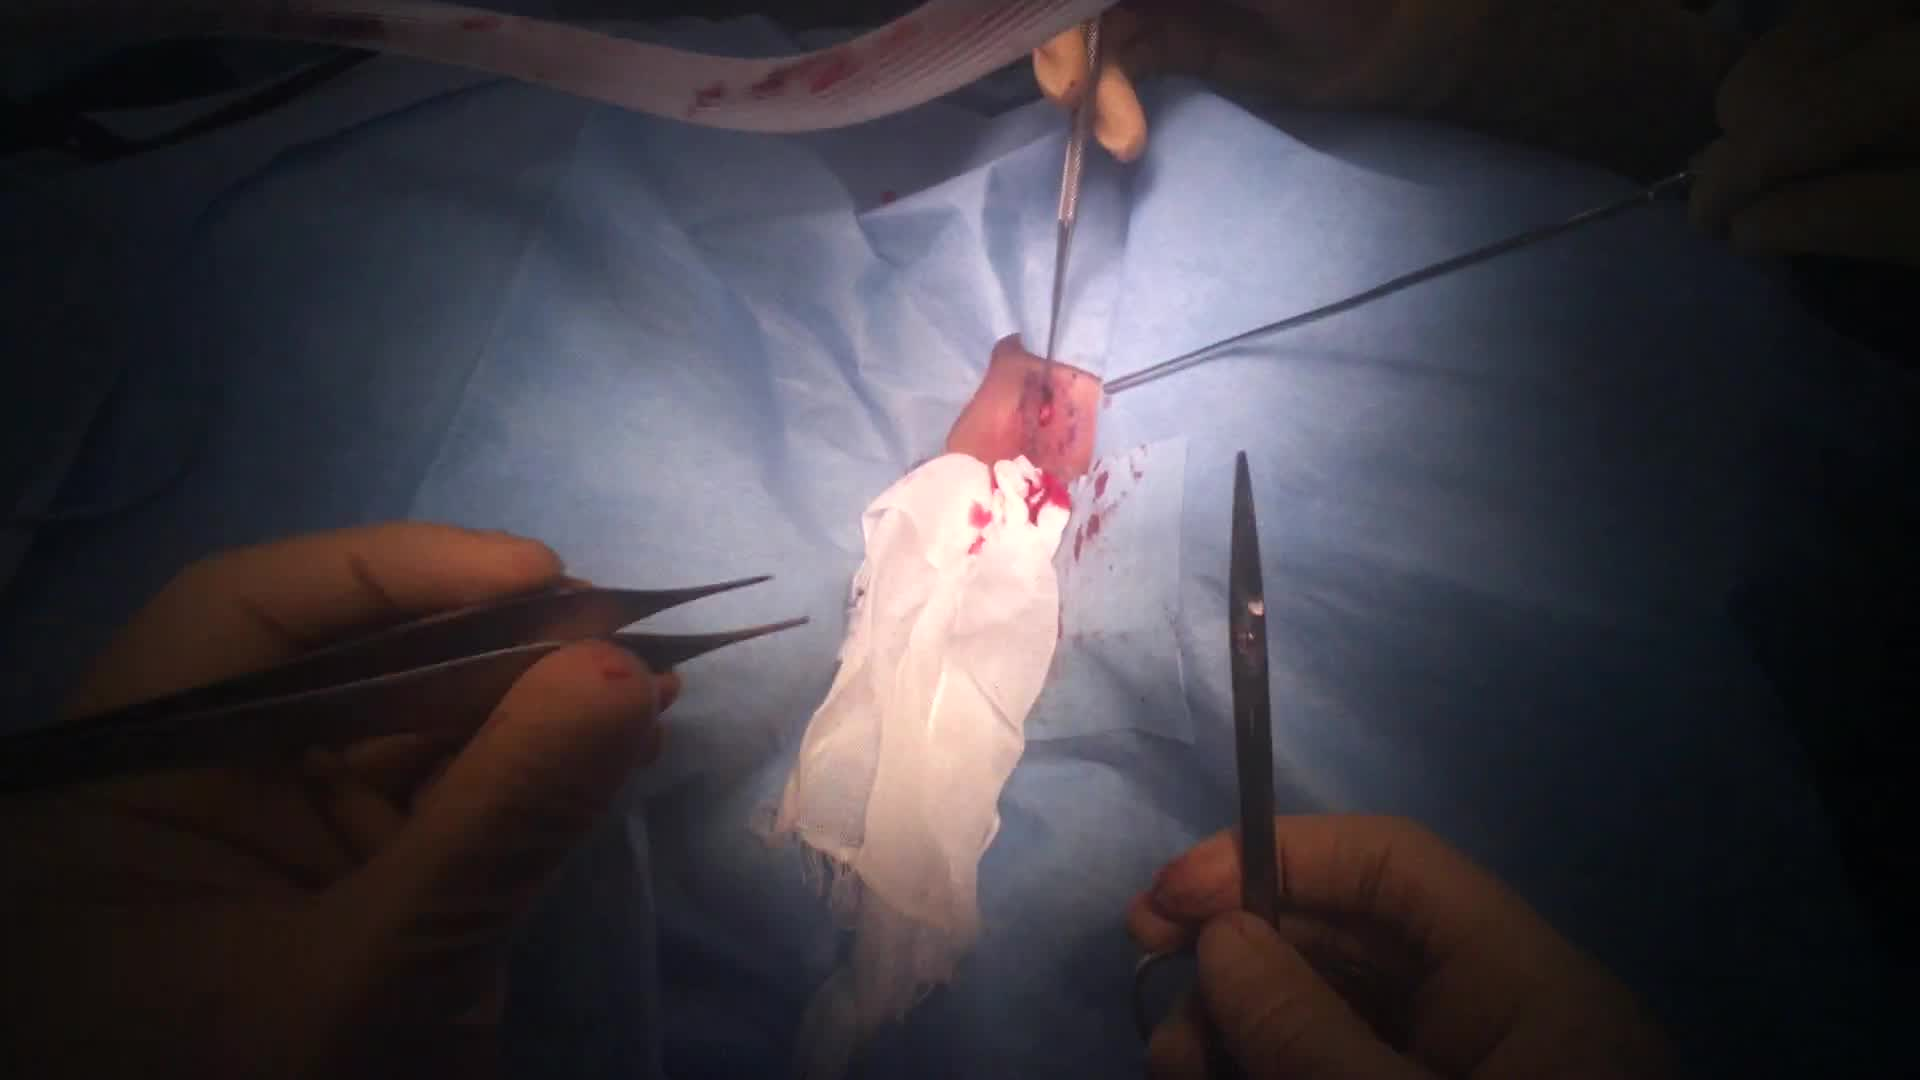
\includegraphics[width=1920\unitlength]{../figures/medvidbench-2767-002.00s.jpg}}%
\linethickness{0.6pt}\color{green}\put(748,1){\framebox(326,631){}}\end{picture}\endgroup\hskip2pt
\VideoStripFrame{../figures/medvidbench-2767-014.00s.jpg}\hskip2pt
\VideoStripFrame{../figures/medvidbench-2767-016.00s.jpg}\hskip2pt
\VideoStripFrame{../figures/medvidbench-2767-030.00s.jpg}}
\end{VideoStrip}
\noindent\VideoStripLabel{2 s}\hspace{2pt}%
\VideoStripLabel{14 s}\hspace{2pt}%
\VideoStripLabel{16 s}\hspace{2pt}%
\VideoStripLabel{30 s}\par
\fontsize{8}{9.5}\selectfont Shared anchor and later frames. The green box at 2 seconds identifies the queried gauze; later frames are shown without additional boxes.
\end{center}
\begin{MessageBox}{black!3}{User message: Question (Task type: Region captioning)}
\begin{Trajectory}
[...] From 2.0 seconds to 32.0 seconds, what is the object doing in the region given by the bounding box at 2.0 seconds? [...]
\end{Trajectory}
\end{MessageBox}
\noindent\textbf{Case 3: Cover the requested interval before describing the action.}
\begin{ExecutionBox}{black!55}{black!6}{VideoSpy$^{\mathbf{0}}$ (Base)}
\raggedright
\begin{MessageBox}[agent message]{dialogueblue}{Round 1: Agent message}
\begin{Trajectory}
name: frame_inspect  arguments: {"query": "What object is in the bounding box at 2.0 seconds and what is it doing?", "timestamps": [2.0]}
\end{Trajectory}
\end{MessageBox}
\begin{MessageBox}[other message]{experienceyellow}{Round 1: Tool message (frame\_inspect)}
\begin{Trajectory}
[...] - The exact action (e.g., pressing, holding, moving) is static in this single frame. [...]
\end{Trajectory}
\end{MessageBox}
\begin{MessageBox}[agent message,frame hidden,borderline={1pt}{0pt}{changeaccent,dash pattern=on 3pt off 2pt},colbacktitle=red!4]{dialogueblue}{Round 2: Agent message}
\noindent\textcolor{changeaccent}{\textbf{Stops at the anchor frame}}\par
\begin{Trajectory}
The object in the bounding box at 2.0 seconds is a blood-stained surgical sponge or gauze resting on the blue surgical drape.
\end{Trajectory}
\end{MessageBox}
\end{ExecutionBox}

% \pagebreak
\begin{ExecutionBox}[breakable,title after break={VideoSpy$^{\mathcal{E}}$ (Skill+Memory, continued)}]{violet!50!black}{experiencepurple}{VideoSpy$^{\mathcal{E}}$ (Skill+Memory)}
\raggedright
\noindent{\footnotesize Select task and domain Skill; retrieve relevant Memory $\rightarrow$ append to system prompt.}\par
\begin{MessageBox}[loaded skill]{experiencepurple}{System prompt: Loaded Skill}
\begin{Trajectory}[highlightlines={3,11},highlightcolor=yellow!25]
region_caption:
**Recommended approach:**
1. **Anchor-then-Track:** Inspect the bounding-box timestamp to identify the object, then use `clip_skim` over the full interval to observe its continuous action.
2. **Resolve Identity Conflicts:** If tools conflict on object type (e.g., forceps vs. scissors), inspect distinct frames to verify physical features (blades vs. jaws) rather than repeating the same query.
3. **Leverage Visual Cues:** Use specific instrument features (e.g., cables, handle color) to infer function (e.g., cautery vs. grasping) when generic descriptions are insufficient.
Domain:
**Recommended approach:** Verify temporal scope and action boundaries using targeted frame inspections; distinguish similar actions by specific mechanical cues (e.g., instrument type, tissue state).
region_caption:
**Pitfalls to avoid:**
1. **Duplicate Loops:** Never repeat a tool call with identical timestamps/queries after a "Duplicate" response. Stop and summarize if evidence is sufficient.
2. **Premature Convergence:** Do not lock onto a single interpretation (e.g., "grasping") if other observations suggest a different function (e.g., "cutting"). Verify the action against the object's physical design.
3. **Over-Interpretation:** Distinguish between repositioning/lifting and actual removal/extraction; do not infer a completed action (e.g., "removed") from a single frame of movement without confirming the object's final state.
Domain:
**Pitfalls to avoid:** Do not infer completed actions or full procedures from coarse overviews or generic knowledge; confirm transitions and final states with direct visual evidence.
\end{Trajectory}
\end{MessageBox}
\begin{MessageBox}[loaded skill]{experiencepurple}{System prompt: Loaded Memory}
\begin{Trajectory}
Historical reasoning case:
Past problem: Determine the specific action of the object in the bounding box at 148s throughout the 148s-200s interval.
Action taken: frame_inspect({"timestamps":[148],"query":"Identify the object in the bounding box region at 148 seconds and what it is doing."}); clip_skim({"end_time":200,"query":"Track the object in the bounding box region (surgical retractor) from 148s to 200s and describe what it is doing.","start_time":148})
Reported result: The object is a surgical retractor held by a gloved hand, actively retracting tissue to maintain exposure of the incision site.

[...]
\end{Trajectory}
\end{MessageBox}
\begin{MessageBox}[agent message,frame hidden,borderline={1pt}{0pt}{changeaccent,dash pattern=on 3pt off 2pt},colbacktitle=red!4]{dialogueblue}{Round 2: Agent message}
\noindent\textcolor{changeaccent}{\textbf{After identifying the gauze, inspect 2--32 seconds}}\par
\begin{Trajectory}
name: clip_skim  arguments: {"query": "Track the object in the bounding box region from 2.0 seconds to 32.0 seconds and describe what it is doing.", "start_time": 2.0, "end_time": 32.0}
\end{Trajectory}
\end{MessageBox}
\begin{MessageBox}[other message]{experienceyellow}{Round 2: Tool message (clip\_skim)}
\begin{Trajectory}
[...] - At 30.0s, the gauze is briefly seen again as the surgeon wipes the area. [...]
\end{Trajectory}
\end{MessageBox}
\begin{MessageBox}[agent message,frame hidden,borderline={1pt}{0pt}{changeaccent,dash pattern=on 3pt off 2pt},colbacktitle=red!4]{dialogueblue}{Round 3: Agent message}
\noindent\textcolor{changeaccent}{\textbf{Describe the observed function across the interval}}\par
\begin{Trajectory}
The object is a blood-stained surgical gauze pad that is intermittently used to absorb and clear blood from the surgical field between 2.0 and 32.0 seconds.
\end{Trajectory}
\end{MessageBox}
\end{ExecutionBox}

\paragraph{What changes.}
Base answers from a single frame. With the anchor-then-track Skill and historical case loaded, the evolved agent inspects 2--32 seconds and describes intermittent blood clearing, matching the reference's functional description. The factual Memory identifies gauze at the anchor; the clip inspection supplies evidence of later use. One additional visual call raises tokens from 9,345 to 18,811.
% Displayed message indices: base 1,2,3,4; skill_memory 0,4,5,6. Evolved Round 1 and finalization omitted.
% Frames: metadata sample 2767, sequence indices 1,7,8,15 at 0.5 fps.
% Anchor bbox [748,448,1074,1079] on the original 1920x1080 frame, drawn in LaTeX only.
\bigskip
\subsection{MedVidBench Sample 5550: Reusing a method to stop earlier}
\label{app:medvid_cvs_efficiency}
\begin{center}
\begin{VideoStrip}
\hbox{\VideoStripFrame{../figures/medvidbench-5550-000.00s.jpg}\hskip2pt
\VideoStripFrame{../figures/medvidbench-5550-010.00s.jpg}\hskip2pt
\VideoStripFrame{../figures/medvidbench-5550-020.00s.jpg}\hskip2pt
\VideoStripFrame{../figures/medvidbench-5550-039.00s.jpg}}
\end{VideoStrip}
\noindent\VideoStripLabel{0 s}\hspace{2pt}%
\VideoStripLabel{10 s}\hspace{2pt}%
\VideoStripLabel{20 s}\hspace{2pt}%
\VideoStripLabel{39 s}\par
\fontsize{8}{9.5}\selectfont Shared frames from the 40-second sequence. Both executions match the reference scores of (0, 0, 0).
\end{center}
\begin{MessageBox}{black!3}{User message: Question (Task type: CVS assessment)}
\begin{Trajectory}
[...] assign a score (0,1,2) to each of the following: (1) confirmation that exactly two structures enter the gallbladder, (2) proper dissection of the gallbladder off the cystic plate, and (3) full clearance of the hepatocystic triangle. [...]
\end{Trajectory}
\end{MessageBox}
\noindent\textbf{Case 4: Preserve the correct answer while avoiding a duplicate loop.}
\begin{ExecutionBox}{black!55}{black!6}{VideoSpy$^{\mathbf{0}}$ (Base)}
\raggedright
\begin{MessageBox}[other message]{experienceyellow}{Round 5: Tool message (frame\_inspect)}
\begin{Trajectory}
[...] - Two structures: 0 (not clearly visible or separated)
- Cystic plate: 0 (not properly dissected)
- Hepatocystic triangle: 0 (not fully cleared) [...]
\end{Trajectory}
\end{MessageBox}
\begin{MessageBox}[agent message,frame hidden,borderline={1pt}{0pt}{changeaccent,dash pattern=on 3pt off 2pt},colbacktitle=red!4]{dialogueblue}{Round 6: Agent message}
\noindent\textcolor{changeaccent}{\textbf{Repeats the Round 5 request}}\par
\begin{Trajectory}
name: frame_inspect  arguments: {"query": "Inspect the gallbladder neck and cystic plate interface at the latest possible time in the video to see if the dissection is complete and the two structures are clearly visible.", "timestamps": [39.0, 39.5, 39.667]}
\end{Trajectory}
\end{MessageBox}
\begin{MessageBox}[other message]{experienceyellow}{Round 6: Tool message (frame\_inspect)}
\begin{Trajectory}
[...] Duplicate `frame_inspect` inspection skipped because it already succeeded. STOP repeating this request. [...]
\end{Trajectory}
\end{MessageBox}
\begin{MessageBox}[agent message]{dialogueblue}{Round 17: Agent final answer}
\begin{Trajectory}
Two structures: 0, Cystic plate: 0, Hepatocystic triangle: 0
\end{Trajectory}
\end{MessageBox}
\end{ExecutionBox}
\begin{ExecutionBox}[breakable,title after break={VideoSpy$^{\mathcal{E}}$ (Skill+Memory, continued)}]{violet!50!black}{experiencepurple}{VideoSpy$^{\mathcal{E}}$ (Skill+Memory)}
\raggedright
\noindent{\footnotesize Select task and domain Skill; retrieve relevant Memory $\rightarrow$ append to system prompt.}\par
\begin{MessageBox}[loaded skill]{experiencepurple}{System prompt: Loaded Skill}
\begin{Trajectory}[highlightlines={4,5,13},highlightcolor=yellow!25]
cvs_assessment:
**Recommended approach:**
Evaluate each CVS criterion independently against specific visual evidence.
For "two structures," require clear separation of the cystic duct and artery; a single indistinct bundle or obscured view scores 0.
For "triangle clearance," active dissection or visible fat/fibrous tissue means the criterion is not met (score 0), regardless of progress.
Do not infer success from the presence of surgical instruments or the general context of cholecystectomy.

Domain:
**Recommended approach:** Verify temporal scope and action boundaries using targeted frame inspections; distinguish similar actions by specific mechanical cues (e.g., instrument type, tissue state).

cvs_assessment:
**Pitfalls to avoid:**
Do not let a positive overview or final-frame inspection override negative evidence from intermediate frames. If any frame shows the triangle is not free of tissue or structures are not distinct, the score must reflect that failure. Avoid assuming that "advanced dissection" equals "CVS achieved"; strict anatomical criteria must be visually confirmed in the specific frames inspected.

Domain:
**Pitfalls to avoid:** Do not infer completed actions or full procedures from coarse overviews or generic knowledge; confirm transitions and final states with direct visual evidence.
\end{Trajectory}
\end{MessageBox}
\begin{MessageBox}[loaded skill]{experiencepurple}{System prompt: Loaded Memory}
\begin{Trajectory}
Historical reasoning case:
Past problem: Determine if the hepatocystic triangle is fully cleared and if exactly two structures enter the gallbladder, as initial overview suggested success but later coarse inspection was inconclusive.
Action taken: frame_inspect({"query":"Look closely at the hepatocystic triangle and the base of the gallbladder. Are exactly two structures (cystic duct and cystic artery) clearly visible entering the gallbladder? Is the gallbladder fully separated from the cystic plate? Is the triangle completely cleared of fat and tissue?","timestamps":[40,45,50,55]})
Reported result: Frame inspection at 40-55s revealed that the triangle is not completely cleared (residual fat/tissue) and the two structures are not clearly visible entering the gallbladder, contradicting the initial positive assessment.

[...]
\end{Trajectory}
\end{MessageBox}
\begin{MessageBox}[agent message,frame hidden,borderline={1pt}{0pt}{changeaccent,dash pattern=on 3pt off 2pt},colbacktitle=red!4]{dialogueblue}{Round 2: Agent message}
\noindent\textcolor{changeaccent}{\textbf{Adapt the historical checklist to the current clip}}\par
\begin{Trajectory}
name: frame_inspect  arguments: {"query": "Inspect the base of the gallbladder and the hepatocystic triangle. Are exactly two structures (cystic duct and cystic artery) clearly visible entering the gallbladder? Is the gallbladder fully separated from the cystic plate? Is the triangle completely cleared of fat and tissue?", "timestamps": [0, 10, 20, 30]}
\end{Trajectory}
\end{MessageBox}
\begin{MessageBox}[other message]{experienceyellow}{Round 3: Tool message (frame\_inspect)}
\begin{Trajectory}
[...] - Frame 29.667s: The dissection continues, but the base of the gallbladder is still not clearly visible. The hepatocystic triangle is not fully cleared. [...]
\end{Trajectory}
\end{MessageBox}
\begin{MessageBox}[agent message,frame hidden,borderline={1pt}{0pt}{changeaccent,dash pattern=on 3pt off 2pt},colbacktitle=red!4]{dialogueblue}{Round 4: Agent message}
\noindent\textcolor{changeaccent}{\textbf{Stop after current-clip verification}}\par
\begin{Trajectory}
[...] Two structures: 0, Cystic plate: 0, Hepatocystic triangle: 0 [...]
\end{Trajectory}
\end{MessageBox}
\end{ExecutionBox}

\paragraph{What changes.}
CVS assessment (Critical View of Safety scoring) requires specialized surgical knowledge and fine-grained anatomical judgment~\citep{su2026medgrpo}. Here, evolution reuses a domain-specific inspection strategy from historical execution experience. The historical case provides a three-criterion inspection query. The evolved run adapts its timestamps to the current clip, checks the final frames, and stops with the correct $(0,0,0)$ answer. Base reaches the same answer after repeating its fifth request in Rounds 6--16 and receiving 11 duplicate rejections. Visual calls fall from 5 to 3, rounds from 17 to 5, and tokens from 103,633 to 32,669 (68.5\% fewer). This case supports more efficient reuse of an inspection strategy.
% Displayed message indices: base 11,12,13,35; skill_memory 0,4,7,8.
% Frames: metadata sample 5550, sequence indices 0,30,60,117 at 3 fps.
